\chapter{Grover's Search: Amplitude Amplification}\label{ch:grover}
\begin{center}\small\textit{Searching an unsorted database of size $N$: classically $N/2$ tries, quantumly $\sqrt{N}$.}\end{center}

\section{Intuition: Rotating Toward the Needle}
You have $N=2^n$ items, one is marked. An oracle can tell you ``yes/no'' for any item, but you have no sorted order to exploit. Classically you must try $\Theta(N)$ items. Grover's idea: prepare equal superposition over all $N$, then repeatedly (a) flip the phase of the marked item and (b) reflect about the average amplitude. Each iteration rotates the state by a fixed angle toward the marked item. After about $\tfrac{\pi}{4}\sqrt{N}$ rotations you are almost certainly at the answer.

Geometrically the dynamics lives in a 2-D plane spanned by $\lvert w\rangle$ (winner) and $\lvert r\rangle$ (rest). Grover is a rotation in that plane.

\section{The Oracle and Diffusion}
Let $M=1$ marked item $w$, $N=2^n$. Define
\begin{equation}
\lvert w\rangle\quad\text{and}\quad
\lvert r\rangle=\tfrac1{\sqrt{N-1}}\sum_{x\neq w}\lvert x\rangle,\qquad
\lvert s\rangle=H^{\otimes n}\lvert0\rangle=\tfrac1{\sqrt N}\sum_x\lvert x\rangle.
\end{equation}
Write $\lvert s\rangle=\sin\theta\lvert w\rangle+\cos\theta\lvert r\rangle$ where $\sin\theta=1/\sqrt N$.

Oracle $O$ flips phase of the winner: $O\lvert w\rangle=-\lvert w\rangle$, $O\lvert r\rangle=\lvert r\rangle$. Diffusion $D=2\lvert s\rangle\langle s\rvert-I$ reflects about $\lvert s\rangle$. Grover iterate $G=D\cdot O$ rotates by $2\theta$ in the $\{ \lvert r\rangle,\lvert w\rangle\}$ plane.

\begin{center}
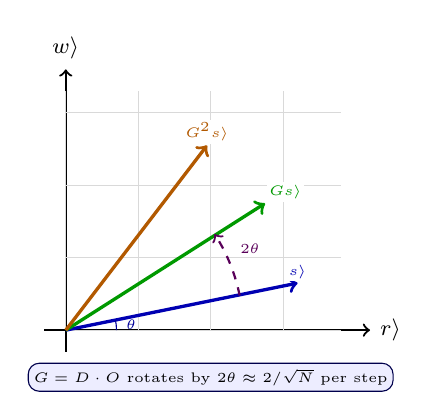
\begin{tikzpicture}[scale=0.92,font=\footnotesize]
  % Grover plane rotation
  \draw[->, thick] (-0.3,0)--(4.2,0) node[right] {$\lvert r\rangle$};
  \draw[->, thick] (0,-0.3)--(0,3.6) node[above] {$\lvert w\rangle$};
  \draw[gray!30] (0,0) grid (3.8,3.3);
  % s vector
  \draw[->, very thick, blue!70!black] (0,0)--(3.2,0.65) node[above, font=\tiny, fill=white, inner sep=1pt] {$\lvert s\rangle$};
  \draw[blue!60!black] (0.7,0) arc (0:11.5:0.7) node[midway, right, font=\tiny] {$\theta$};
  % after one iteration
  \draw[->, very thick, green!60!black] (0,0)--(2.75,1.75) node[above right, font=\tiny, fill=white, inner sep=1pt] {$G\lvert s\rangle$};
  \draw[->, very thick, orange!70!black] (0,0)--(1.95,2.55) node[above, font=\tiny, fill=white, inner sep=1pt] {$G^2\lvert s\rangle$};
  % arc showing rotation by 2theta
  \draw[->, thick, violet!70!black, dashed] (2.4,0.48) arc (11.5:33:2.45) node[midway, above right, font=\tiny] {$2\theta$};
  \node[fill=blue!7, draw=blue!30!black, rounded corners, inner sep=2pt, font=\tiny] at (2.0,-0.65) {$G=D\cdot O$ rotates by $2\theta\approx2/\sqrt N$ per step};
\end{tikzpicture}
\end{center}

\begin{center}
\begin{tikzpicture}[scale=0.88,font=\footnotesize]
  \draw[thick] (0,0.6)--(7.0,0.6);
  \draw[thick] (0,0)--(7.0,0);
  \node[left, font=\tiny] at (0,0.6) {$\lvert x\rangle$};
  \node[left, font=\tiny] at (0,0) {$\lvert y\rangle$};
  % H block
  \draw[fill=blue!15, thick] (0.6,0.25) rectangle (1.3,0.95) node[midway, font=\tiny] {$H^{\otimes n}$};
  % Oracle box
  \draw[fill=orange!15, thick] (1.9,-0.3) rectangle (3.0,0.9) node[midway, align=center, font=\tiny] {$O$\\{\tiny flip $w$}};
  % Diffusion box
  \draw[fill=green!15, thick] (3.5,-0.3) rectangle (4.7,0.9) node[midway, align=center, font=\tiny] {$D$\\{\tiny $2|s\rangle\langle s|-I$}};
  \draw[fill=violet!10, thick, dashed] (1.75,-0.45) rectangle (4.85,1.05) node[above, font=\tiny] {$G=D\,O$ $\times k$ times};
  % dots
  \node at (5.3,0.3) {$\cdots$};
  % meter
  \draw[fill=blue!12, thick] (5.9,0.3) rectangle (6.5,0.9);
  \draw (6.2,0.45) arc (180:0:0.11);
  \draw[->, thick] (6.2,0.45)--(6.31,0.68);
  \node[font=\tiny, fill=white, inner sep=1pt] at (3.3,1.25) {Grover iterate};
  \node[fill=green!7, draw=green!30!black, rounded corners, inner sep=2pt, font=\tiny] at (3.3,-1.0) {Prepare $\lvert s\rangle$, repeat $G$ about $\tfrac{\pi}{4}\sqrt N$ times, measure};
\end{tikzpicture}
\end{center}

\section{Optimal Number of Iterations}

After $k$ iterates,
\begin{equation}
G^k\lvert s\rangle=\sin\bigl((2k+1)\theta\bigr)\lvert w\rangle+\cos\bigl((2k+1)\theta\bigr)\lvert r\rangle,
\end{equation}
so success probability is $\sin^2((2k+1)\theta)$.

\begin{theorem}[Grover optimum]
Optimum $k^\star\approx\frac{\pi}{4\theta}-\frac12\approx\frac{\pi}{4}\sqrt N$ gives $\Pr[\text{success}]\approx1$. Overshooting rotates past $\lvert w\rangle$ and success falls. For $M$ marked items, $\sin\theta=\sqrt{M/N}$ and $k^\star\approx\frac{\pi}{4}\sqrt{N/M}$.
\end{theorem}

Grover is optimal: any quantum algorithm needs $\Omega(\sqrt{N/M})$ queries (BBBV bound). Speedup is quadratic, not exponential, but applies to any unstructured search ---  $10^6$ items: $500\,000\to 785$ queries.

\begin{center}
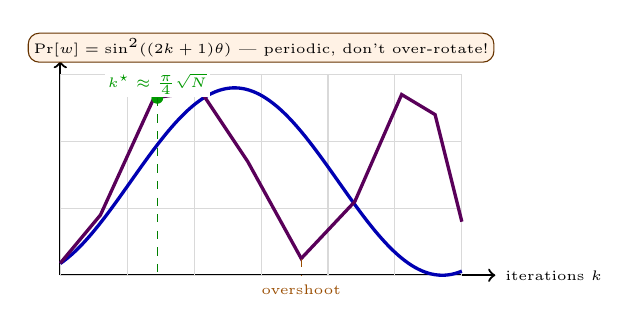
\begin{tikzpicture}[scale=0.85,font=\footnotesize]
  \draw[->, thick] (0,0)--(6.5,0) node[right, font=\tiny] {iterations $k$};
  \draw[->, thick] (0,0)--(0,3.2) node[above, font=\tiny] {$\Pr[w]$};
  \draw[gray!30] (0,0) grid (6,3);
  % sine squared curve
  \draw[very thick, blue!70!black, domain=0:6, samples=120, smooth] plot (\x,{2.8*pow(sin((2*\x+1)*14.5),2)});
  % Actually plot sin^2((2k+1)theta) with theta ~ 1/sqrt(16)=14.5deg
  % Use simpler manual curve
  \draw[very thick, violet!70!black] (0,0.18)--(0.6,0.9)--(1.4,2.65)--(2.1,2.75)--(2.8,1.7)--(3.6,0.25)--(4.4,1.1)--(5.1,2.7)--(5.6,2.4)--(6.0,0.8);
  \fill[green!60!black] (1.45,2.65) circle (2.5pt) node[above, font=\tiny, fill=white, inner sep=1pt] {$k^\star\approx\frac{\pi}{4}\sqrt N$};
  \draw[dashed, green!50!black] (1.45,2.65)--(1.45,0);
  \draw[dashed, orange!60!black] (3.6,0.25)--(3.6,0) node[below, font=\tiny] {overshoot};
  \node[fill=orange!10, draw=orange!40!black, rounded corners, inner sep=2pt, font=\tiny] at (3.0,3.4) {$\Pr[w]=\sin^2((2k+1)\theta)$ --- periodic, don't over-rotate!};
\end{tikzpicture}
\end{center}

\section{Amplitude Amplification}
Grover generalizes: given algorithm $A$ with success probability $p$, amplification needs $O(1/\sqrt p)$ repetitions versus $O(1/p)$ classically. Reflection about $A\lvert0\rangle$ replaces Hadamards. This underpins quantum counting, collision finding, and nested Grover for optimization.


\section{Geometric View and Fixed-Point Variants}
Amplitude amplification can be seen as two reflections whose product is a rotation. Reflection $O$ about $\lvert r\rangle$ flips the $\lvert w\rangle$ component; $D$ reflects about $\lvert s\rangle$. Composition of two reflections is a rotation by twice the angle between their axes. This is why Grover is exact analog of classical ``inversion about mean'' used in some randomized algorithms, but with coherent phases.

Fixed-point search (Yoder--Low--Chuang) avoids overshoot by using varying phases: instead of $-1$ flips, use $e^{i\phi_j}$ tuned so success probability monotonically increases to $1-O(\delta)$ without needing to know $M$ exactly. The price is a slightly larger constant factor.

\begin{example}[When $M$ is unknown]
If $M$ is unknown, run exponential probing: try $k=1,2,4,8,\dots$ Grover steps with random restarts. Expected queries remain $O(\sqrt{N/M})$. Quantum counting (phase estimation on $G$) estimates $M$ first to $\pm\sqrt M$ accuracy using $O(\sqrt N)$ queries.
\end{example}

\section{Applications Beyond Search}
Grover speeds up any brute-force check: SAT with $n$ variables ($N=2^n$) from $O(2^n)$ to $O(2^{n/2})$, collision finding $O(N^{1/3})$, and element distinctness $O(N^{2/3})$. In cryptanalysis it halves symmetric key strength: AES-128 offers $\sim64$ bits quantum security, hence AES-256 is recommended post-quantum symmetric standard.


\section{Error Analysis and Reality}
Grover assumes perfect oracle and diffusion. With depolarizing error $p$ per gate, fidelity after $k\sim\sqrt N$ steps decays as $(1-p)^{k\cdot G}$ where $G$ gates per iteration. Mitigation via amplitude amplification with error-aware scheduling helps but ultimately fault tolerance is needed for large $N$. Near-term Grover demonstrations on $n\le5$ show the predicted sinusoidal success probability even with NISQ noise, validating the rotation picture.


\section{Beyond Unstructured Search: Structured Variants}
Quantum walk search generalizes Grover to graphs: find a marked vertex with $O(\sqrt{HT})$ where $HT$ is hitting time. For grids and trees this can beat Grover when structure allows faster traversal. The framework unifies Grover, element distinctness, and triangle finding ($O(n^{1.25})$ vs.\ classical $O(n^2)$).


\section{Variations and History}
Grover (1996) discovered the algorithm by thinking about reflections; Boyer--Brasard--Hoyer--Tapp (1998) analyzed $M$ marks and unknown $M$. Zalka proved exact optimality. Amplitude amplification (Brassard et al., 2002) generalized to any $A$ with success $p$. Today Grover is a subroutine in quantum walks, nested search, and QAOA initialization, not a standalone database search, because $O(\sqrt N)$ oracle calls still require $O(\sqrt N)$ coherent quantum memory accesses (QRAM) for large $N$.


\section{Python: Grover Simulation}

\begin{lstlisting}[language=Python]
import numpy as np

def grover_sim(N, w, steps):
    """Simulate Grover for N items, marked w, for given steps."""
    n = int(np.log2(N))
    s = np.ones(N, dtype=complex)/np.sqrt(N)  # |s>
    # Oracles
    O = np.eye(N, dtype=complex); O[w,w] = -1
    D = 2*np.outer(s, s.conj()) - np.eye(N)
    G = D @ O
    psi = s.copy()
    for _ in range(steps):
        psi = G @ psi
    probs = np.abs(psi)**2
    return psi, probs

N, w = 16, 5
for k in [0,1,2,3,4]:
    _, p = grover_sim(N, w, k)
    print(f"k={k}  P(w)={p[w]:.3f}  max P={p.max():.3f}")

# Optimal k ~ pi/4 * sqrt(N)
k_opt = int(np.round(np.pi/4*np.sqrt(N)))
print("k_opt", k_opt, "P(w) at opt:", grover_sim(N,w,k_opt)[1][w])
\end{lstlisting}

\begin{lstlisting}[language=Python]
# Scaling demo: classical vs quantum queries
import math
for N in [16, 64, 256, 1024]:
    classical = N//2
    quantum = int(math.pi/4*math.sqrt(N))
    print(f"N={N:4d}  classical ~{classical:4d}  quantum ~{quantum:3d}  speedup {classical/quantum:.1f}x")

# Multiple marked items
N, marked = 16, [3, 7]
M = len(marked)
theta = math.asin(math.sqrt(M/N))
k_opt_M = int(round((math.pi/2 - theta)/(2*theta)))
print(f"\nM={M} N={N} theta={theta:.3f} k_opt={k_opt_M}")
\end{lstlisting}


\section{Query Lower Bounds}
The BBBV theorem shows no quantum algorithm uses $o(\sqrt N)$ queries for unstructured search. Proof uses hybrid argument: after $t$ queries, amplitudes for oracles differing at one point differ by at most $O(t/\sqrt N)$; distinguishing needs $t=\Omega(\sqrt N)$. Thus Grover is asymptotically optimal. For exact success, $\lceil\frac{\pi}{4\theta}-\frac12\rceil$ queries are necessary and sufficient. Variants with multiple marked items meet $\Omega(\sqrt{N/M})$ similarly.

\begin{remark}
Grover does not imply NP$\subseteq$BQP with speedup $2^{n/2}$ for $k$-SAT is still exponential. Quadratic helps but does not collapse NP. For structured problems, better-than-Grover speedups need structure (e.g., lattice sieving, backtracking with quantum walks).
\end{remark}


\begin{remark}[Optimality sketch]
BBBV hybrid argument: let $\lvert\psi_t^f\rangle$ be state after $t$ queries to $f$. For $f,f_w$ differing at $w$, $\|\lvert\psi_t^f\rangle-\lvert\psi_t^{f_w}\rangle\|\le2t/\sqrt N$. Distinguishing needs $\Omega(\sqrt N)$. Grover is tight; for $M$ marks, $\sqrt{N/M}$.
\end{remark}

\begin{example}[Fixed-point search]
Standard Grover overshoots if $k>k^\star$. Fixed-point version uses phases $\phi_j$ in $R_s(\phi)=I-(1-e^{i\phi})\lvert s\rangle\langle s\rvert$. Chebyshev-chosen $\phi_j$ makes success monotonic, reaching $1-\delta$ without knowing $M$, paying $O(\log1/\delta)$ overhead.
\end{example}

\begin{remark}[Quantum counting]
Phase estimation on $G$ estimates $\theta$ with $\sin\theta=\sqrt{M/N}$, hence $M$ to $O(\sqrt M)$. Cost $O(\sqrt N)$. This enables exponential probing when $M$ unknown with expected optimal cost.
\end{remark}

\section{Exercises}
\begin{exercise}
For $N=4$, $w=3$, simulate Grover by hand: write $\lvert s\rangle$, apply $O$, then $D$, and show one iteration finds $w$ with probability $1$.
\end{exercise}
\begin{exercise}
Prove $D= H^{\otimes n}(2\lvert0\rangle\langle0\rvert-I)H^{\otimes n}$ and explain why reflection about $\lvert0\rangle$ can be built from $X$ gates and a multi-controlled $Z$.
\end{exercise}
\begin{exercise}
Derive $k^\star\approx\frac{\pi}{4}\sqrt{N/M}$ for $M$ marked items. What is $k^\star$ for $N=10^6$, $M=10$? What happens if you run twice as many iterations?
\end{exercise}
\begin{exercise}
Show Grover provides no advantage when $M=N/4$: compute $k^\star$ and explain why one iteration already yields $\Pr=1$ but classical also needs $O(1)$.
\end{exercise}
\begin{exercise}
Implement amplitude amplification: given unitary $A$ that prepares $\sqrt p\lvert good\rangle+\sqrt{1-p}\lvert bad\rangle$, simulate $O(1/\sqrt p)$ Grover steps and plot success probability vs.\ steps for $p=0.05$.
\end{exercise}
